\subsection{Introduction to Atomic Force Microscopy}
The Atomic Force Microscope (AFM) is a type of Scanning Probing Microscope\cite{salapaka2008scanning} developed by Binnig, Quate and Gerbe at IBM, Zurich\cite{PhysRevLett.56.930, eaton2010atomic}. It uses a sharp probe tip to raster-scan a sample's topology and has become a versatile tool\cite{JALILI2004907,SANTOS2004133, goken1999microstructural}. The technique has various applications, for example, in atomic imaging of crystal structures \cite{yu2016atomic} and surface measurements of materials and polymer films \cite{passeri2011indentation,d2012evaluation,dallaeva2014afm, acikgoz2020speed,zeng2017novel}. In addition, AFM can image under natural conditions, such as in aqueous solutions and in real-time, allowing imaging of cell dynamics and biological processes. This includes imaging protein unfolding \cite{hughes2016physics} and conformational changes\cite{moody2006atomic}, alongside, characterising microbial surfaces\cite{wright2006application,dufrene2004using}. The ability to image and measure the physical properties of microbial surfaces can give important insight into microbiology, such as improving inhibition and cellular damage produced by antimicrobial compounds\cite{wright2006application, TYAGI2010797}. 

The imaging of AFM is based on detecting atomic forces acting between a sharp probe tip and the surface of a sample. A schematic of an AFM is shown in Figure \ref{fig: AFM mechanism}. A cantilever holds the sharp tip used to probe the sample surface. A laser beam detection system using the position-sensitive photodiode (PSPD) enables the AFM system to monitor and record the deflection of the cantilever. The tip is raster-scanned across the surface of a sample, and interaction between the tip and surface causes deflection. Subsequently, the deflection is processed in the feedback system, designed to compensate for the change in topology and hold the deflective force constant during scanning. The tip deflection is compared to a reference force, producing an error signal that generates the feedback signal. The surface topography is then determined by mapping the contours of equal force\cite{maghsoudy2018review}.

\begin{figure}[H]
    \centering
    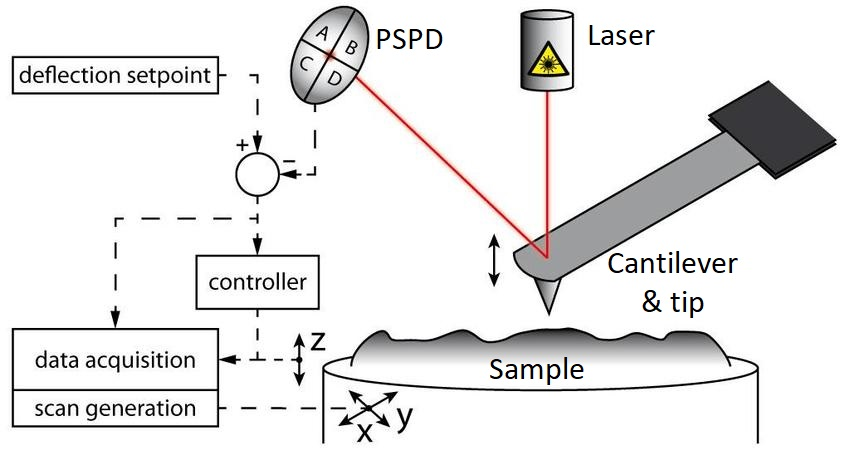
\includegraphics[width=0.75\linewidth]{Figures/Schematic-of-an-atomic-force-microscope.png}
    \caption{Schematic of AFM mechanism from Schitter \textit{et al.}\cite{schitter}}
    \label{fig: AFM mechanism}
\end{figure}

However, as with any experimental technique, AFM has limitations. Various effects can lead to ambiguity in images and image artefacts. A key source of error is a consequence of the resolution being directly dependent on imaging force and the probe geometry \cite{dufrene2002atomic}. Imaging with large forces can dramatically reduce image resolution and damage the surface. Furthermore, probe geometry and its interaction with the sample is important to image contrast \cite{dufrene2002atomic}. As shown in Figure \ref{fig: AFM Convolution}, an AFM image is a convolution of the probe geometry and the sample's topology. Therefore, the tip-sample convolution produces a trace of the tip geometry over the surface, broadening protrusions and narrowing holes in the surface.

\begin{figure}[ht]
\centering

    \begin{subfigure}[t]{0.3\textwidth}
        \centering
        \caption{\label{fig: AFM Convolution}}
        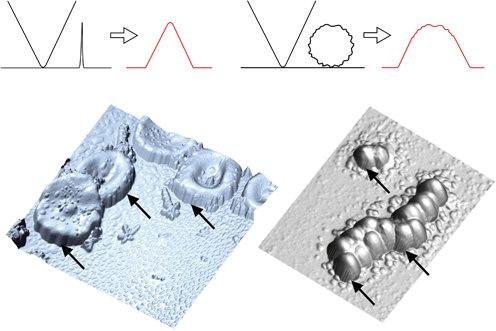
\includegraphics[width=1\linewidth]{Figures/Convolution artefact 2.jpeg}
    \end{subfigure}
    \hfill
    \begin{subfigure}[t]{0.3\textwidth}
        \centering
        \caption{\label{fig: AFM Convolution 2}}
        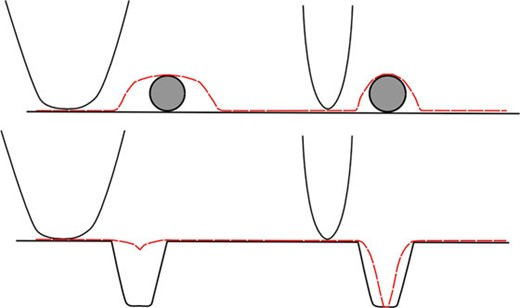
\includegraphics[width=1\linewidth]{Figures/AFM convolution artefact.jpg}
    \end{subfigure} 
    \hfill
    \begin{subfigure}[t]{0.3\textwidth}
        \centering
        \caption{\label{fig: AFM Parachuting}}
        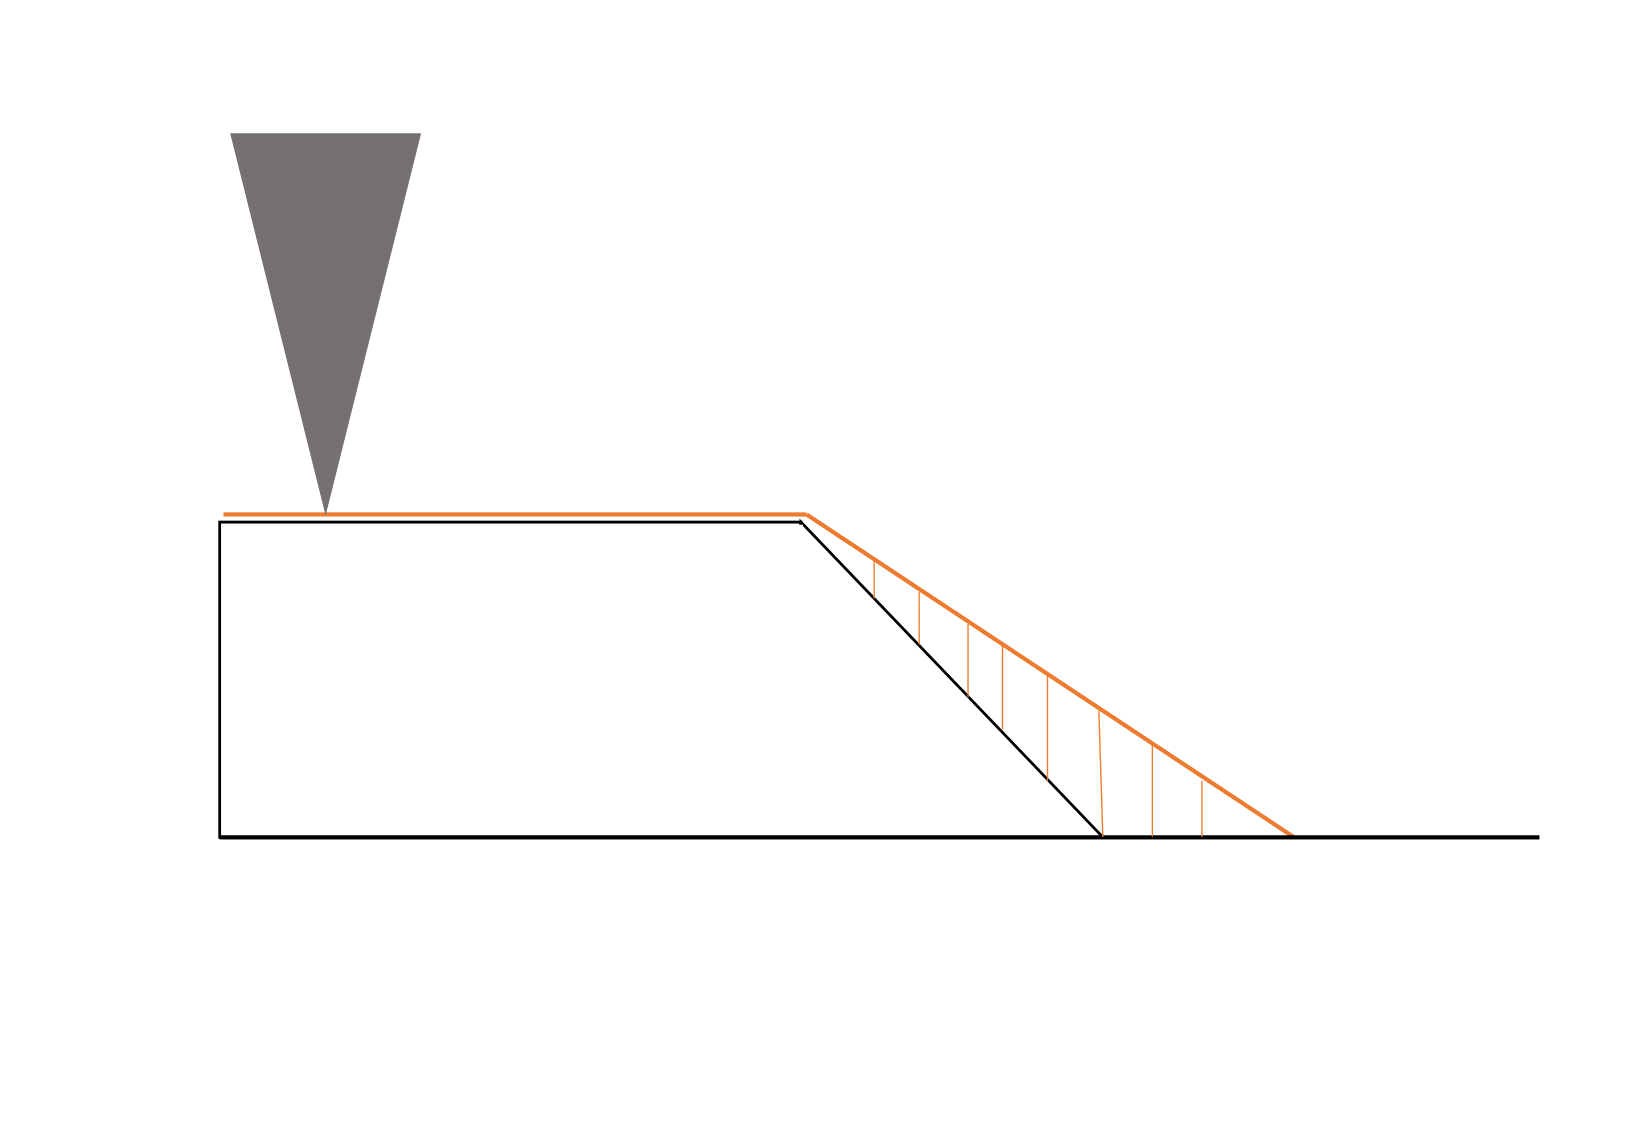
\includegraphics[width=1\linewidth]{Figures/AFM parachuting.png}
    \end{subfigure}

    \caption{\label{fig: AFM Artefacts}Illustrations of typical AFM artefacts taken or adapted from Eaton \& West, Atomic Force Microscopy\cite{eaton2010atomic}. (A) Illustration of tip convolution artefact produced in AFM images. (B) Illustration of the widening/narrowing of surface features due to tip convolution. (C) Illustration of an elongated edge due to the parachuting effect. }
    
\end{figure}

Similarly to tip convolution, AFM can produce image artefacts due to tip interaction when scanning over the edge of a surface structure. As the tip loses contact with the sample, the deflective forces diminish over the edge. As a result, the probe must increase scan depth; however, the cantilever descends at a capped rate, so the tip gradually approaches the surface, minimising the risk of over-indenting. This causes a linearly protracted trace of the gradient and produces an elongated edge in the direction of the image scan, as shown in Figure \ref{fig: AFM Parachuting}. This is known as parachuting.

Furthermore, other errors may arise due to environmental surroundings. For example, environmental vibrations can cause the probe to vibrate and produce artefacts and blur. Similarly, thermal drift is produced from prolonged usage, which causes the probe to expand/ contract thermally and produce deviations in the system. In this report, we describe computational simulations of AFM imaging to aid in interpreting images and artefacts. Moreover, we present some quantitative analysis of the compression produced in these simulations to explore the effect of imaging force and tip geometry in AFM imaging.


